% Version 0.2
\documentclass[a4paper]{article}
 
\usepackage[english,german]{babel}
\usepackage[utf8]{inputenc}
\usepackage[T1]{fontenc}
\usepackage{ae}
\usepackage{comment}
\usepackage[bookmarks,bookmarksnumbered]{hyperref}
\usepackage{enumerate}
\usepackage{datetime}
\usepackage[table,xcdraw]{xcolor}
\usepackage{graphicx}

\DeclareGraphicsExtensions{.pdf,.png,.jpg,.jpeg,.gif}
\newcommand{\horrule}[1]{\rule{\linewidth}{#1}} % Create horizontal rule command with 1 argument of height

\author{Gruppe 17}

\title{
	\normalfont
	\normalsize 
	\huge{Pflichtenheft Buchhandlung Schiller}
	\horrule{0.5pt}
	\paragraph{Version: 0.5}
	\paragraph{Status: in Arbeit}
	\paragraph{Stand: \today}
	\horrule{2pt}
}

\begin{document}

\maketitle

\newpage
 
\section*{Zusammenfassung}

\paragraph{Dies ist das Pflichtenheft für das Projekt Buchhandlung Schiller. Dieses Projekt wird durch die Gruppe 17 betreut. Es handelt sich um eine Verkaufsanwendung, welche in Java programmiert wird, Diese Verkaufsanwendung stellt einen Internetauftritt als auch einen Onlineshop für die Buchhandlung Schiller dar. In diesem Pflichtenheft werden die Anforderungen an das Projekt festgeschrieben.}
 
\section*{Historie}

\begin{comment}

|l|l|l|l|l|

\end{comment}

\begin{tabular}{|r|r|c|l|c|}
	\hline
	\rowcolor[HTML]{C0C0C0} 
	Version & Status    & Datum      & Bearbeiter       & Erläuterung    \\ \hline
	0.1     & In Arbeit & 30.10.2014 & Christoph Kepler & Initial Commit \\ \hline
	0.2     & In Arbeit & 01.11.2014 & Christoph Kepler & Diagramme      \\ \hline
	0.3     & In Arbeit & 07.11.2014 & Christoph Kepler & Letzte Punkte  \\ \hline
\end{tabular}

\section*{Reviewnachweis}

\begin{tabular}{|l|l|l|l|}
	\hline
	\rowcolor[HTML]{C0C0C0} 
	Version & Datum      & Reviewer       & Erläuterung    \\ \hline
\end{tabular}

\newpage

% Platzierung des Inhaltsverzeichnisses

\tableofcontents

\newpage
 
\section{Aufgabenstellung und Zielsetzung}

\paragraph{Die Buchhandlung SCHILLER benötigt eine Verkaufsanwendung. Hauptsächlich ist eine Verkaufsanwendung für die Bücher zu implementieren. Jedoch hat der Geschäftsführer noch einige eigene Ideen. 
Die Anwendung benötigt, neben einer Artikelverwaltung auch eine Benutzerverwaltung. Zu jedem Buch muss mindestens der Autor, Verlag, die ISBN und eine kurze Inhaltsbeschreibung gespeichert werden. Eine Abbildung des Buchbundes anzuzeigen, würde die Attraktivität des Verkaufsprogrammes deutlich steigern. Die Bücher der Buchhandlung SCHILLER sind nach Genre in die Kategorien Fiktion, Sachbuch, Unterhaltung, Ratgeber unterteilt. Eine Möglichkeit zu Erweiterung und nachträglichem Hinzufügen weiterer Genres ist wünschenswert. Der Geschäftsinhaber denkt auch über ein Angebot von CDs und DVDs nach. Die Benutzerverwaltung soll einige wichtige Angaben zum Kunden liefern (Name, Kundennummer, Lieferadresse, etc.). 
Als zusätzliches Feature wünscht der Buchhandel SCHILLER sich einen Kalender auf der Homepage, welcher die wöchentlichen Lesungen aufführt, die in den Räumen der Buchhandlung stattfinden. Die Bezahlung der gekauften Bücher erfolgt über Rechnungsversand.}

\section{Fachlicher Überblick}

\paragraph{Um die Aufgabenstellung zu realisieren wird das Java Framework Spring verwendet. Um die Verkaufsaspekte abzudecken, wird zusätzlich das Java Framework Salespoint eingesetzt. Diese beiden Frameworks sollen durch Wiederverwendung den Programmieraufwand so gering wie möglich halten. Die im SWT-Modul gelernten Design-Patterns sollen genutzt werden, um größtmögliche Modularisierung, einfache Erweiterbarkeit und unkomplizierte Wartung zu gewährleisten.}

\paragraph{Die zu erstellende Web Applikation stellt eine Verkaufsanwendung für die Buchandlung SCHILLER dar. Über diese Anwendung sollen Artikel in verschiedenen Kategorien zum Verkauf angeboten werden. Dazu müssen sich die Gäste an dem System mit ihrer korrekten E-Mail-Adresse registrieren. Es werden Rollen auf die einzelnen Nutzer verteilt, welche dadurch spezielle Berechtigungen auf das System erben. Für die verschiedenen Rollen ist es dann möglich ihrer Tätigkeit nach zu gehen. So kann zum Beispiel der Reading Manager die Lesungen in den dafür bereitgestellten Kalender und die Ressource Raum eintragen, solange nicht schon eine Lesung dort vorhanden ist. Der Rechnungsversand erfolgt automatisch als pdf via E-Mail an den Kunden.}

\section{Systemgrenze und Top-Level-Architektur}

\subsection{Kontextdiagramm}

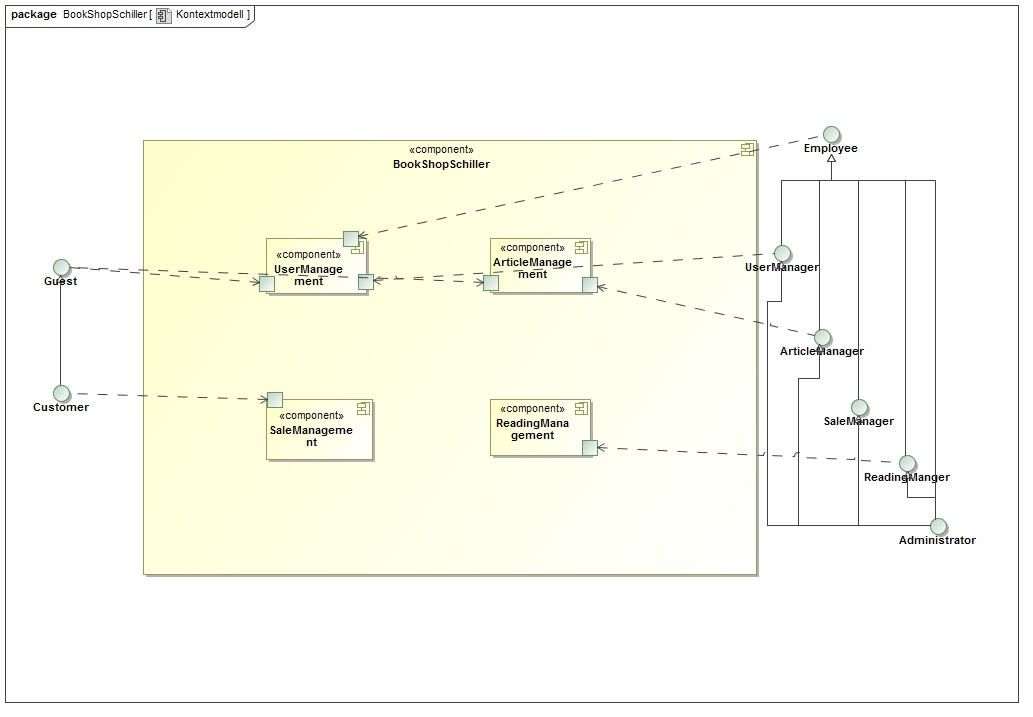
\includegraphics[width=350px]{kontextmodell.jpg}

\subsection{Top-Level-Architektur}

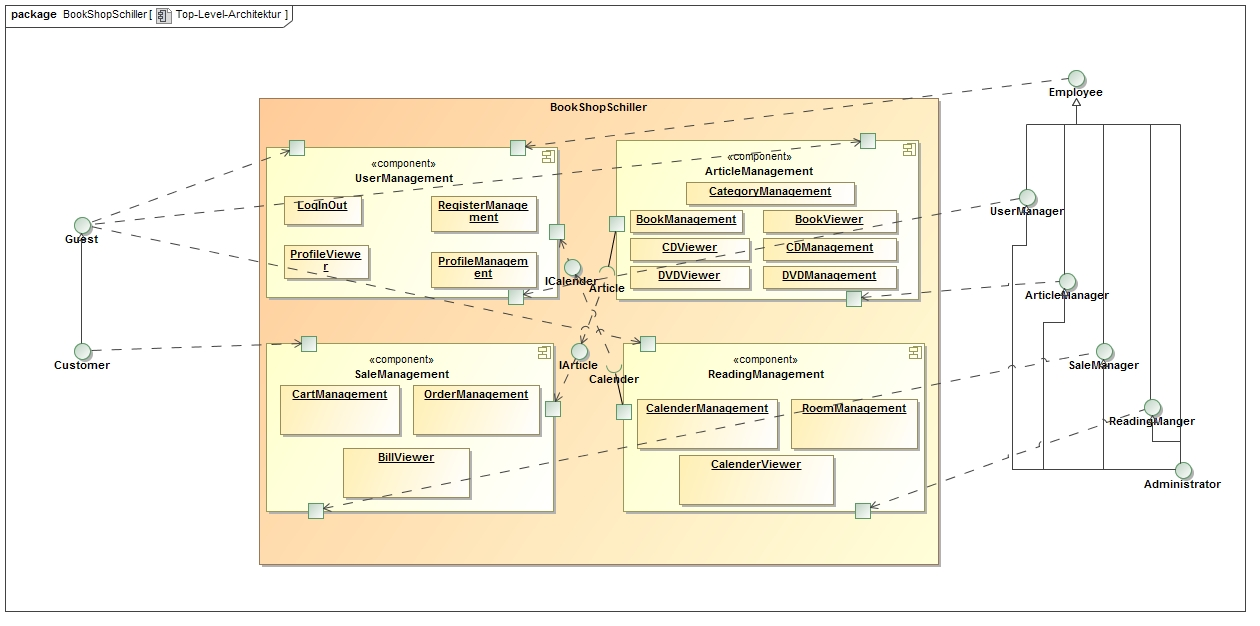
\includegraphics[width=350px]{top-level-architektur.jpg}

\section{Anwendungsfälle}

\subsection{Überblick: Anwendungsfalldiagramm}

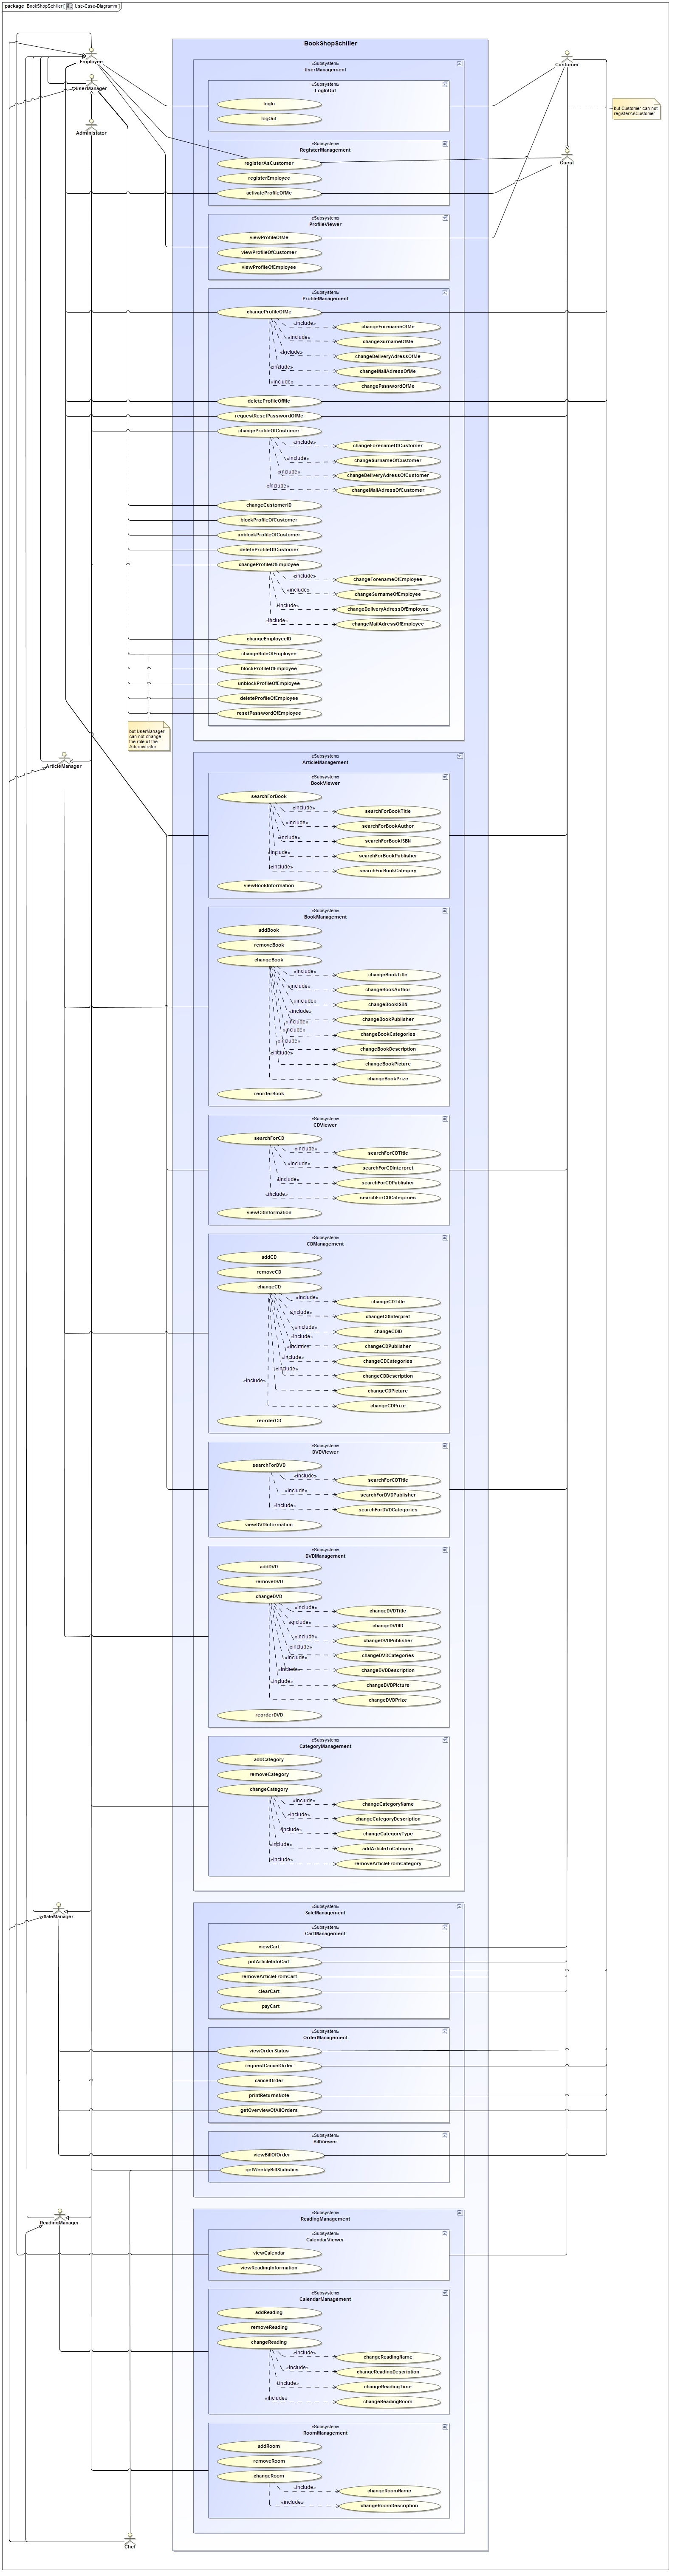
\includegraphics[width=350px]{use-case-diagramm.jpg}

\subsection{Akteure}

\begin{tabular}{|l|l|}
	\hline
	\rowcolor[HTML]{C0C0C0} 
	Name & Beschreibung	\\ \hline
	Guest & Der Guest ist ein unauthentifizierter Nutzer der Anwendung.\\ \hline
	Customer & Der Customer ist ein authentifizierter Nutzer der Anwendung.\\ \hline
	Employee & Der Employee ist ein Mitarbeiter der Firma.\\ \hline
	User Manager & Der User Manager ist der Verwalter von registrierten Nutzern im System.\\ \hline
	Article Manager & Der Article Manager ist der Verwalter vom Artikelbestand im System.\\ \hline
	Reading Manager & Der Reading Manager ist der Verwalter der Lesungen im System.\\ \hline
	Chef & Der Chef stellt den Chef der Firma da.\\ \hline
	Admin/Root/User 0 & Der Admin ist der Nutzer mit allen Rechten.\\ \hline
\end{tabular}

\subsection{Anwendungsfallbeschreibung}

\begin{itemize}
	\item[\textbf{Usermanagement:}]
	\item Login/Logout
	\item Register as user
	\item[\textbf{Userdata:}]
	\item different role management
	\item Manipulate
	\item View own
	\item View costumer
	\item Reset Password
	\item[\textbf{Article Management:}]
	\item View Articles (Books, CD, DVD)
	\item Search articles via different criteria
	\item manipulate article inventory
	\item manipulate categories
	\item[\textbf{Sales Management:}]
	\item
	\begin{itemize}
		\item[\textbf{Cart Management:}]
		\item fill/empty cart
		\item checkout
		\item[\textbf{Order Management:}]
		\item view order
		\item cancel/ get return
		\item[\textbf{Bill Management:}]
		\item view
		\item statistics
	\end{itemize}
	\item[\textbf{Reading Management:}]
	\item view/ manipulate calender
	\item manipulate reading events
	\item manipulate rooms
\end{itemize}

\section{Sequenzdiagramme}

\subsection{Article Management}

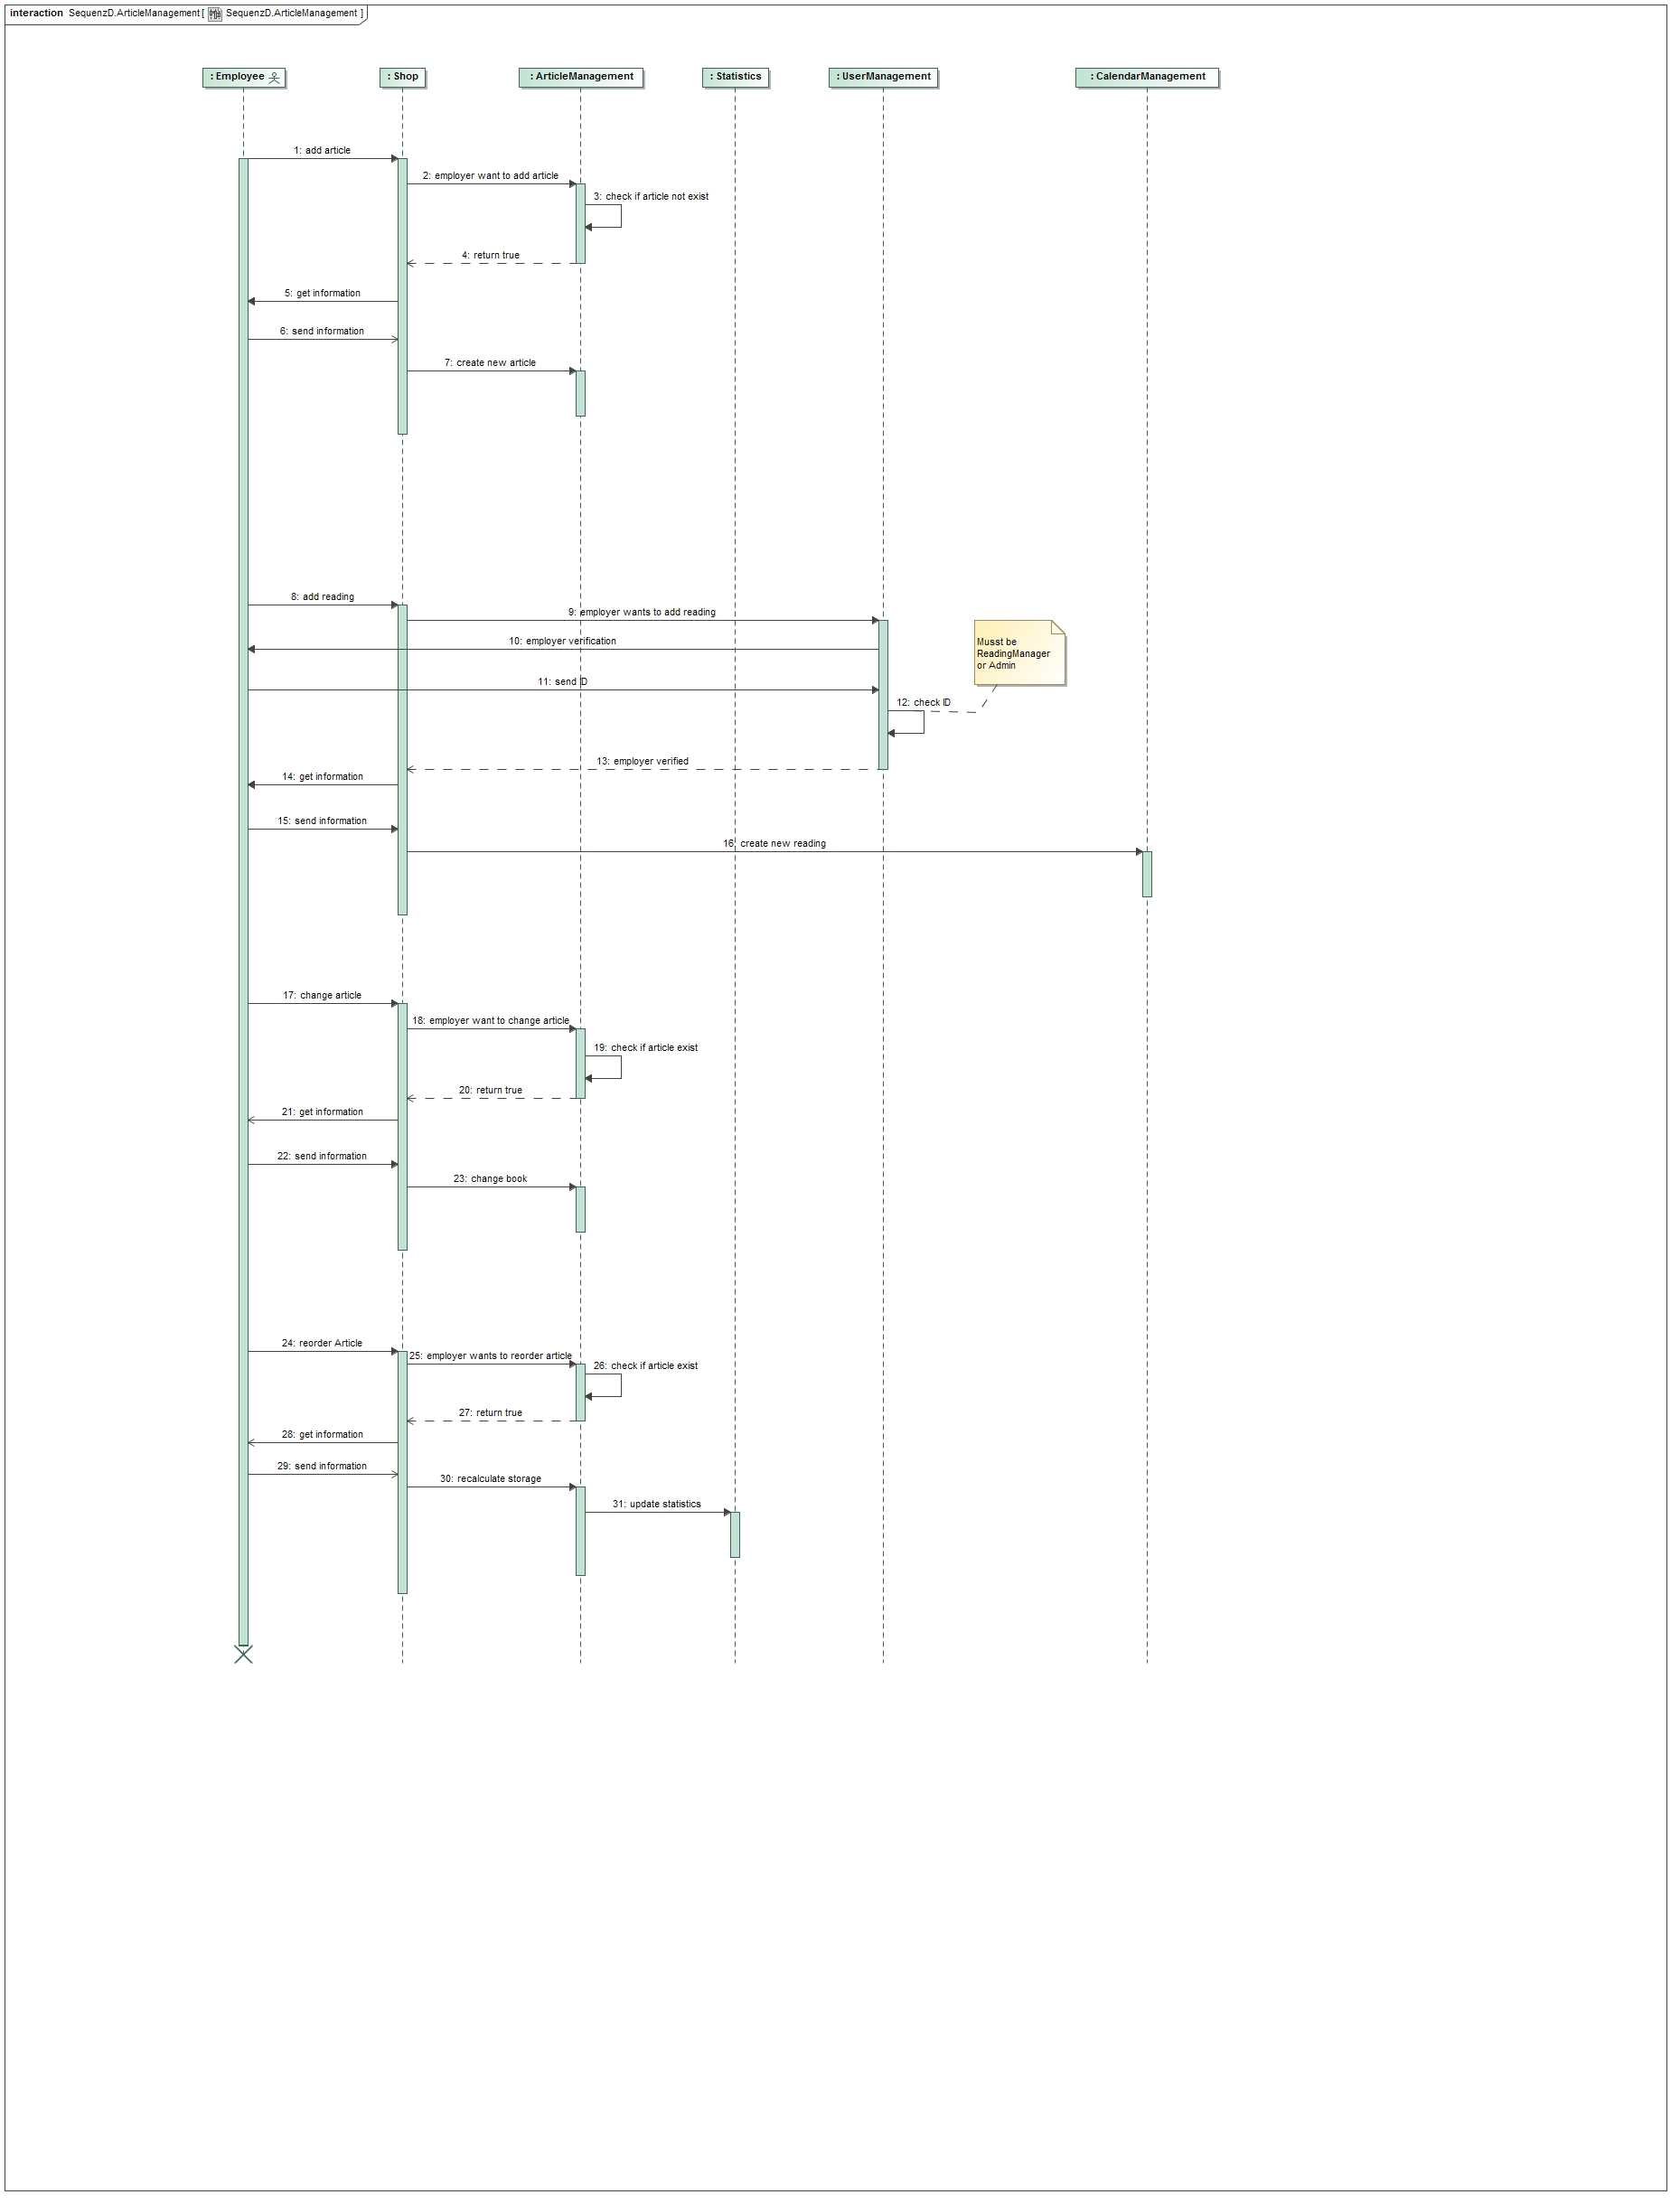
\includegraphics[width=350px]{sd-articlemanagement.jpg}

\subsection{Profile Management}

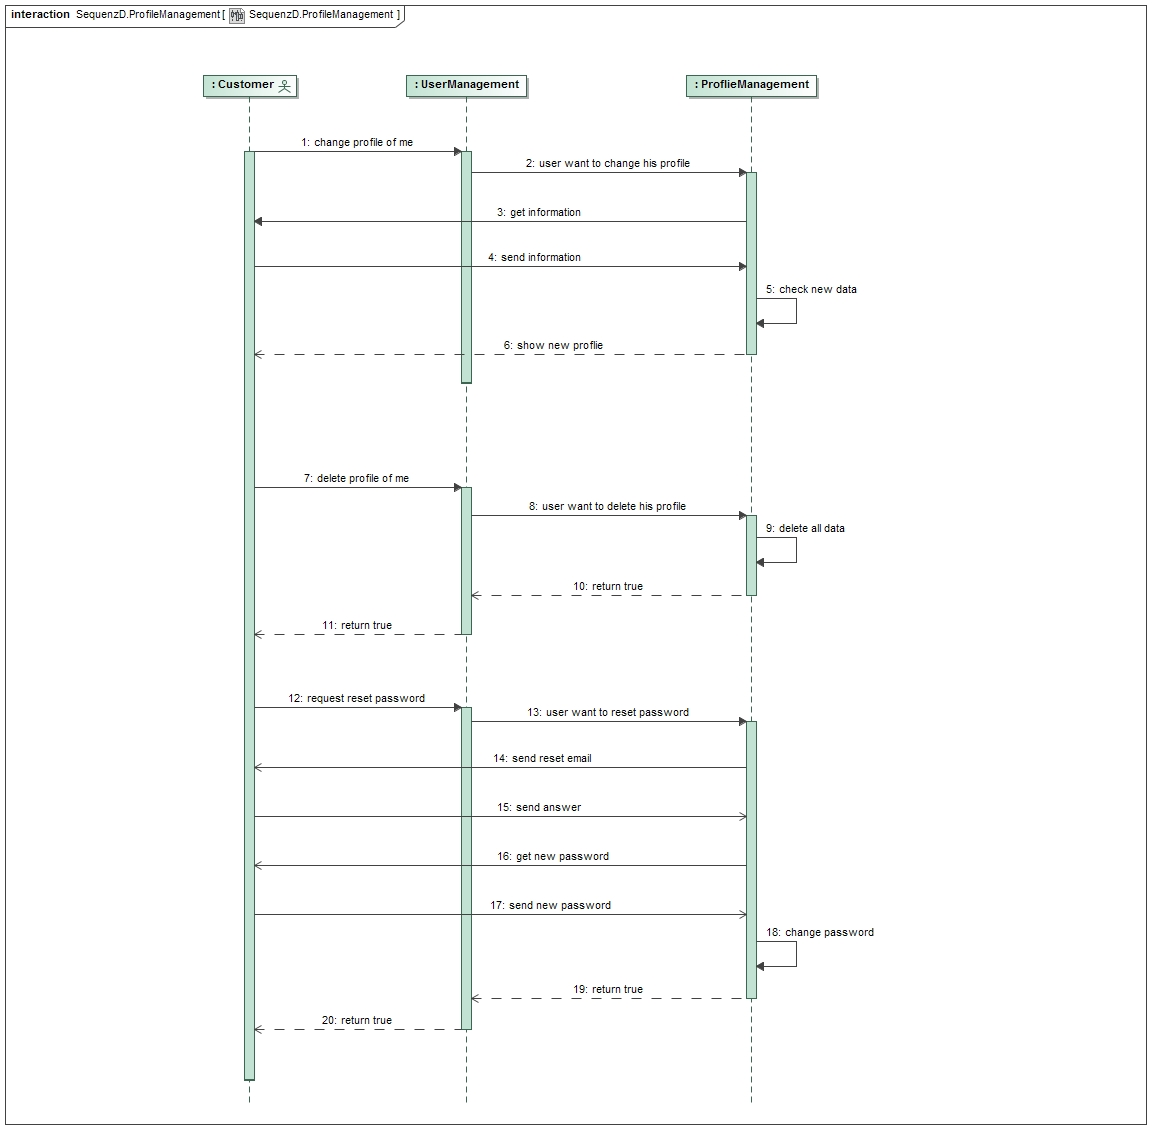
\includegraphics[width=350px]{sd-profilemanagement.jpg}

\subsection{Purchase}

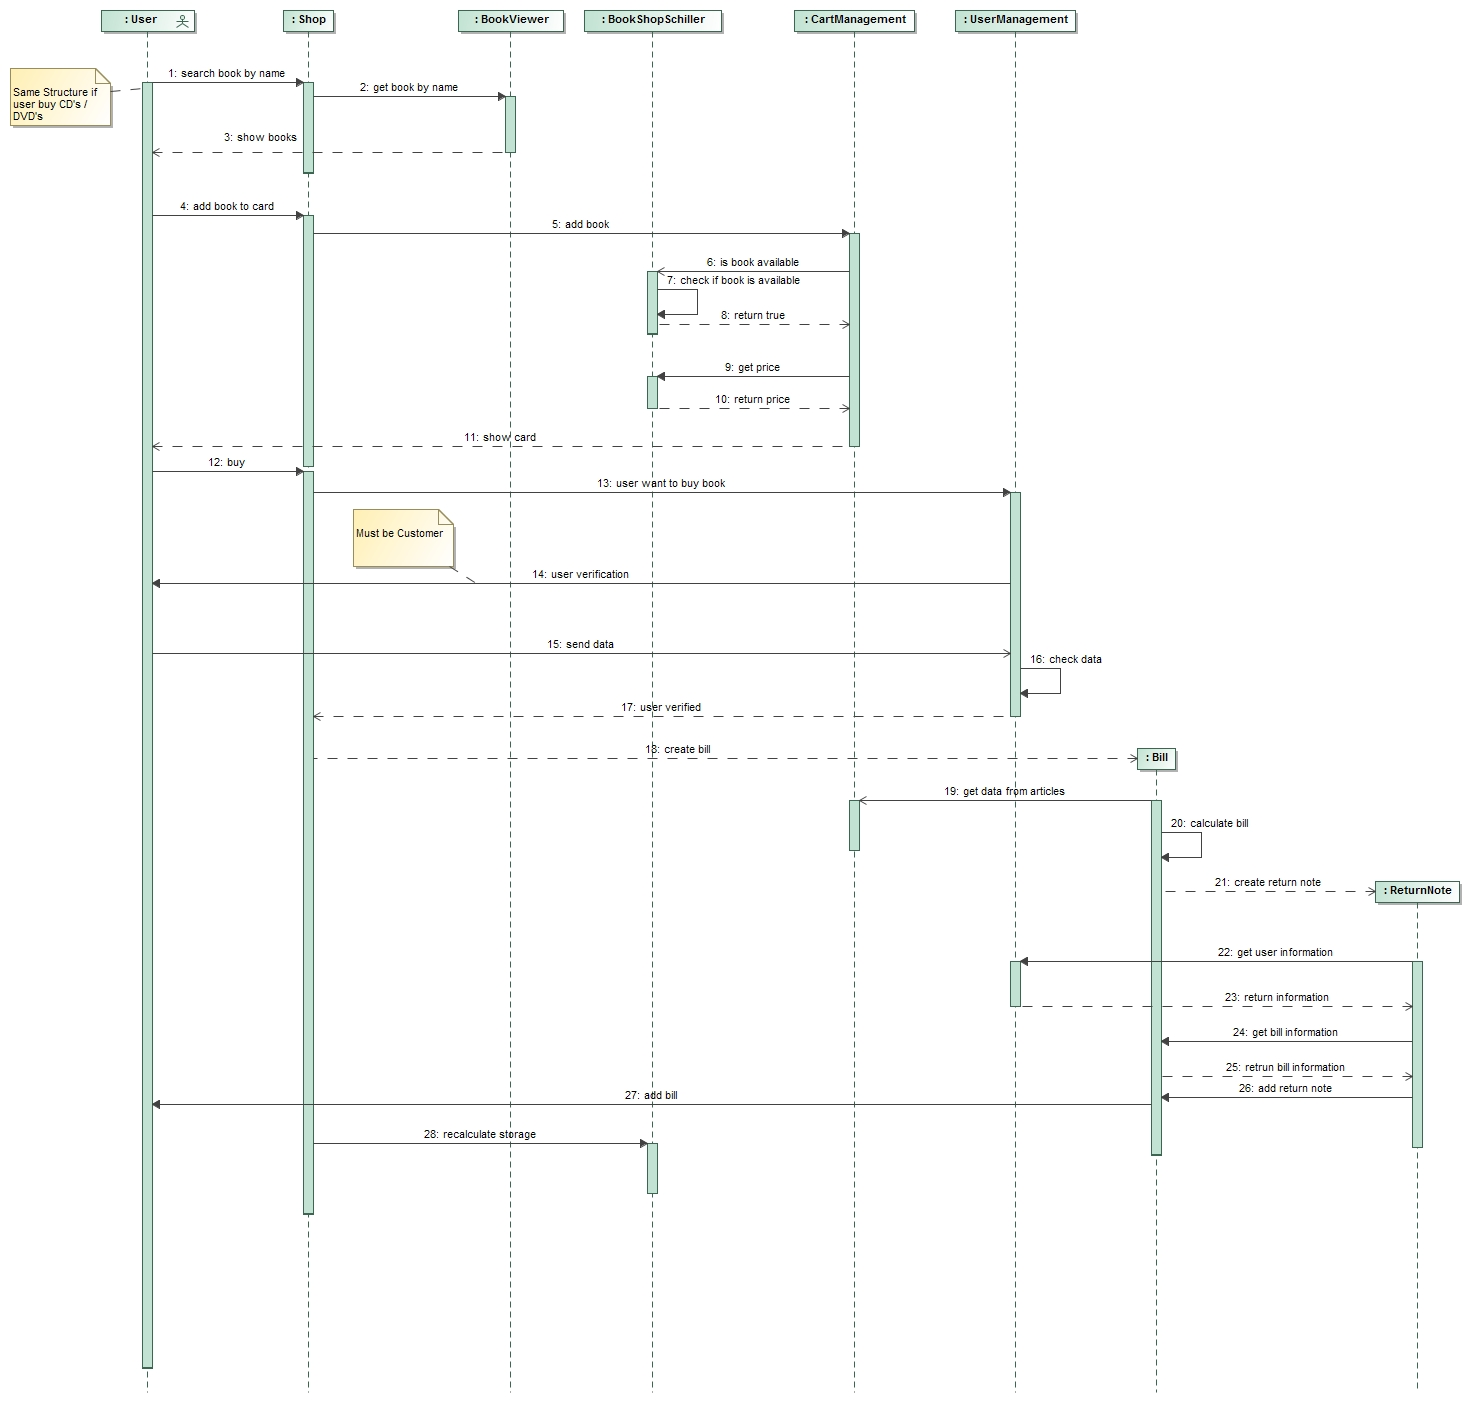
\includegraphics[width=350px]{sd-purchase.jpg}

\subsection{Registration}

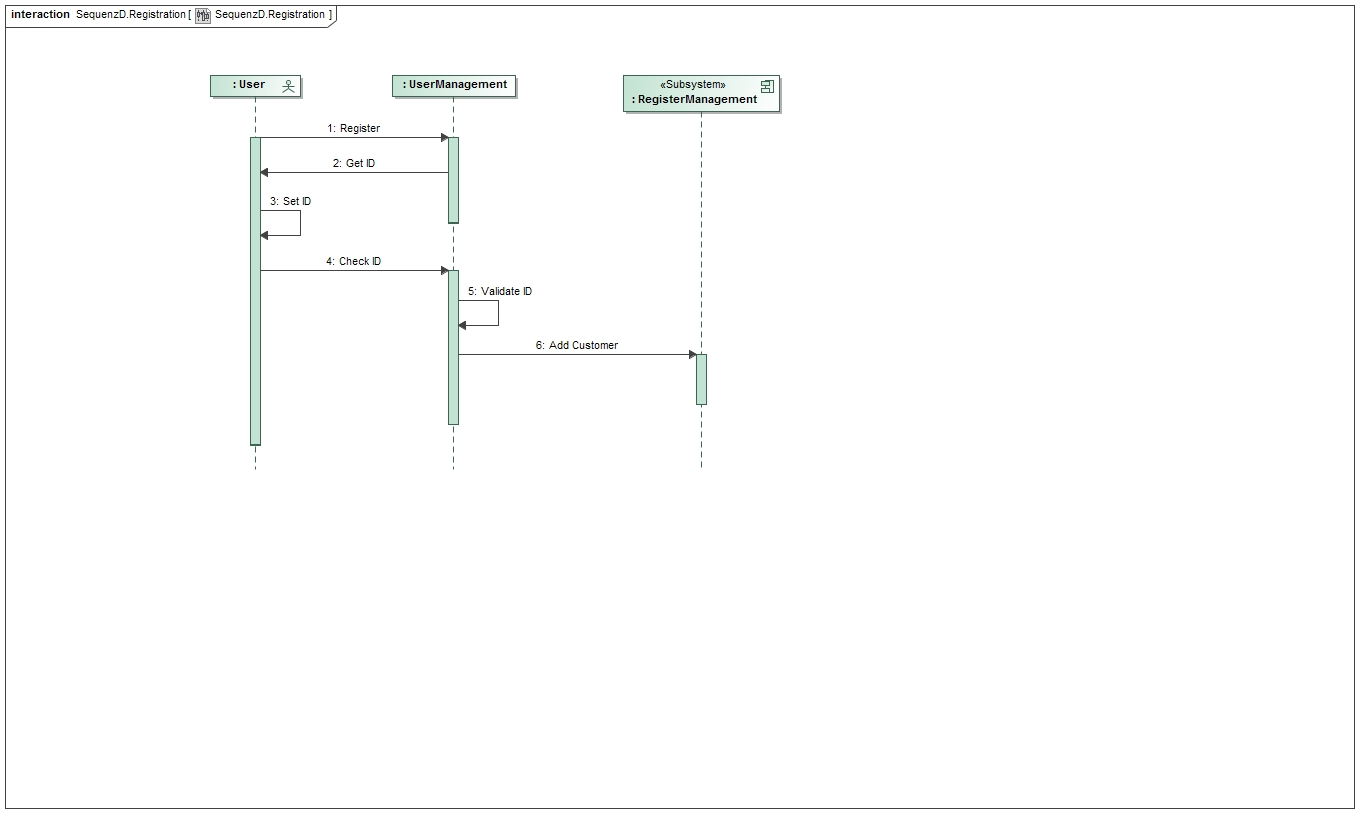
\includegraphics[width=350px]{sd-registration.jpg}

\section{Anforderungen}

\subsection{Musskriterien}

\begin{itemize}
	\item Akteure: Mitarbeiter, nicht eingeloggter Nutzer, eingeloggter Nutzer, Chef,\ Administrator, Personalverwalter
	\item Nutzeraccount kann mehrere Rollen haben
	\item mind. ein Root im System
	\item artikelspezifische Kategorien
	\item Kalender für wöchentliche Lesungen
	\item[Guest kann:]
	\item Artikel suchen
	\item Artikel in Warenkorb legen
	\item nicht kaufen
	\item[Customer kann:]
	\item kaufen
	\item Übersicht über bereits gekaufte Artikel anzeigen
	\item Rechnung online anzeigen lassen und herunterladen
	\item[Employee kann:]
	\item Artikelbestand sehen
	\item ggf. nachbestellen
	\item[User Manager kann:]
	\item Rollen der anderen Nutzer verändern, außer Root
	\item[Chef kann:]
	\item wöchentliche Verkaufsbilanzen anzeigen
	\item[Root kann:]
	\item alles
	\item Kategorien manipulieren
	\item Räume manipulieren
\end{itemize}

\subsection{Kannkriterien}

\begin{itemize}
	\item Meldung, wenn Benutzername bereits vergeben
	\item Meldung, wenn E-Mail syntaktisch nicht richtig
	\item pdf-Rechnung per Mail and den Kunden
	\item Artikel haben verschiedene Kaufs- und Verkaufspreise
\end{itemize}

\subsection{Wunschkriterien}

\begin{itemize}
	\item Möglichkeit Artikel nach Kategorien zu filtern
	\item grafische Visualisierung der Bilanzen (Chart.js)
\end{itemize}

\section{Dialoge (GUI-Prototyp)}

\subsection{Überblick: Dialoglandkarte}

\textit{<Erstellen Sie ein Übersichtsdiagramm, das das Zusammenspiel Ihrer Masken zur Laufzeit darstellt. Also mit welchen Aktionen zwischen den Masken navigiert wird. Die nachfolgende Abbildung zeigt eine an die Pinnwand gezeichnete Dialoglandkarte. Ihre Karte sollte zusätzlich die Buttons/Funktionen darstellen, mit deren Hilfe Sie zwischen den Masken navigieren.>}

\subsection{Dialogbeschreibung}

\textit{
	\begin{enumerate}
		\item[Für jeden Dialog:]
		\item Kurze textuelle Dialogbeschreibung eingefügt: Was soll der jeweilige Dialog? Was kann man damit tun? Überblick?
		\item Maskenentwürfe (Screenshot, Mockup)
		\item Maskenelemente (Ein/Ausgabefelder, Aktionen wie Buttons, Listen, …)
		\item Evtl. Maskendetails, spezielle Widgets
	\end{enumerate}
}

\section{Datenmodell}

\subsection{Überblick: Klassendiagramm}

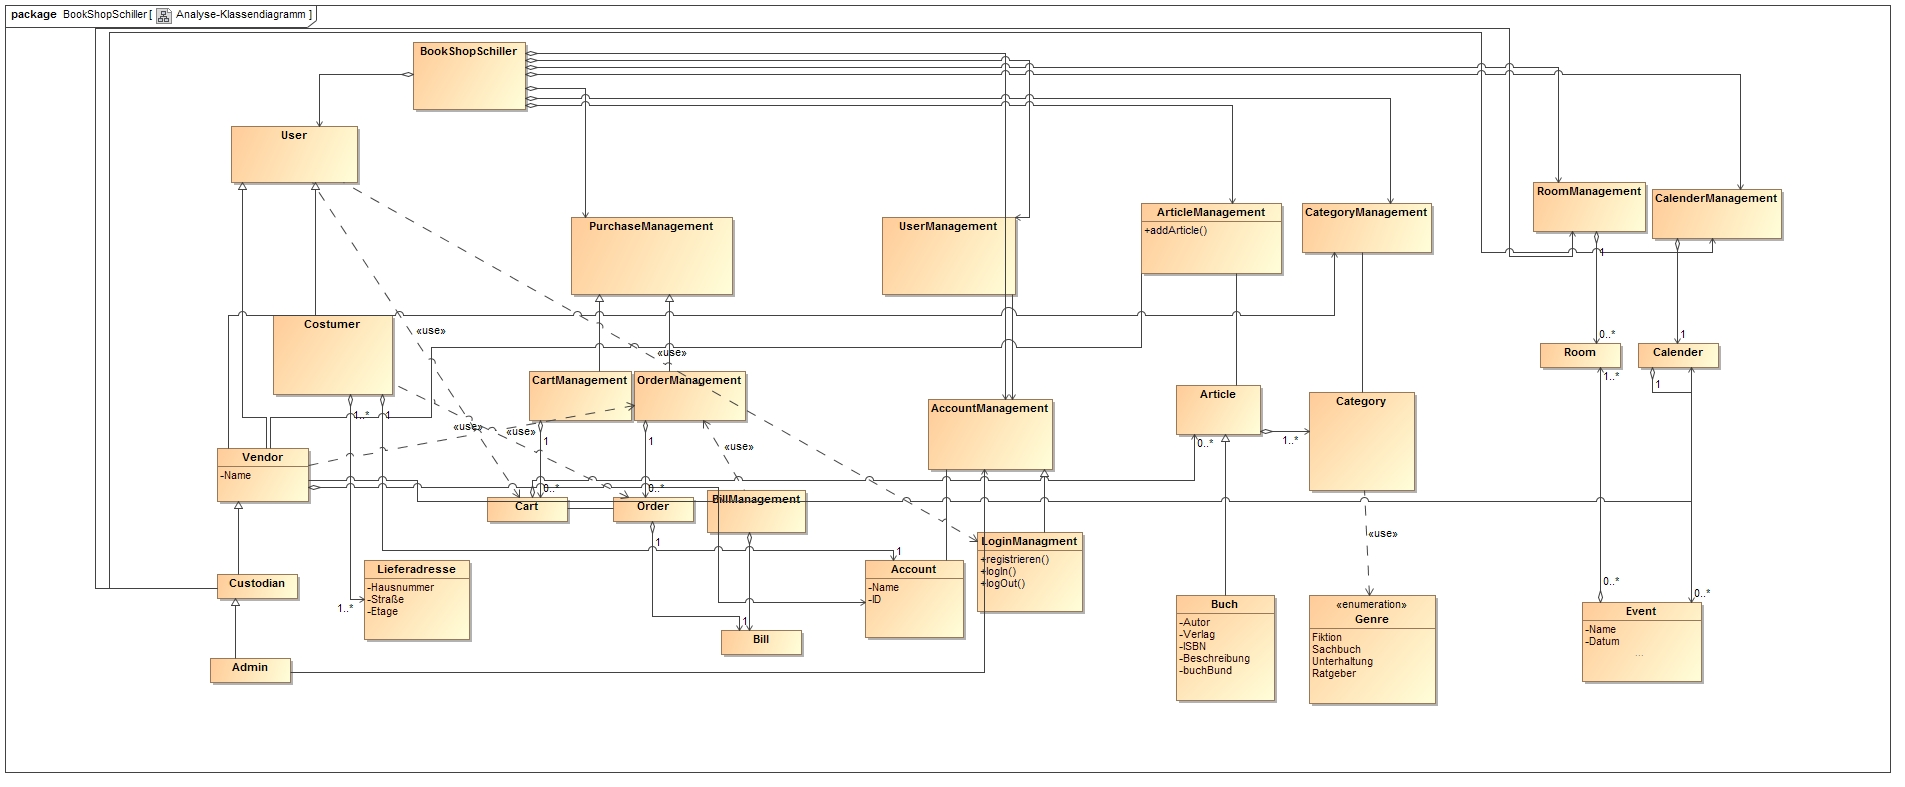
\includegraphics[width=350px]{analyse-klassendiagramm.jpg}

\subsection{Klassen und Enumerationen}

\begin{tabular}{|l|l|}
	\hline
	\rowcolor[HTML]{C0C0C0} 
	Klasse/Enumeration & Beschreibung \\ \hline
	BookShopSchiller &  \\ \hline
	Guest &  \\ \hline
	Costumer &  \\ \hline
	Employee &  \\ \hline
	UserManager &  \\ \hline
	ReadingManager &  \\ \hline
	SaleManager &  \\ \hline
	ArticleManager &  \\ \hline
	Admin &  \\ \hline
	Chef &  \\ \hline
	Lieferadresse &  \\ \hline
	SaleManagement &  \\ \hline
	CartManagement &  \\ \hline
	OrderManagement &  \\ \hline
	Cart &  \\ \hline
	Order &  \\ \hline
	BillViewer &  \\ \hline
	Bill &  \\ \hline
	Account	 &  \\ \hline
	UserManagement  &  \\ \hline
	ProfileManagement &  \\ \hline
	RegisterManagement &  \\ \hline
	ProfileViewer &  \\ \hline
	LogInOut &  \\ \hline
	ArticleManagement &  \\ \hline
	CategoryManagement &  \\ \hline
	BookManagement &  \\ \hline
	DVDManagement &  \\ \hline
	CDManagement &  \\ \hline
	BookViewer &  \\ \hline
	DVDViewer &  \\ \hline
	CDViewer &  \\ \hline
	Article &  \\ \hline
	Category &  \\ \hline
	Book &  \\ \hline
	DVD &  \\ \hline
	CD &  \\ \hline
	Genre <Enumeration> &  \\ \hline
	ReadingManagement &  \\ \hline
	RoomManagement &  \\ \hline
	CalenderManagement &  \\ \hline
	CalenderViewer &  \\ \hline
	Room &  \\ \hline
	Calender &  \\ \hline
	Event &  \\ \hline
\end{tabular}


\section{Akzeptanzfälle}

\textit{
<Mithilfe von Akzeptanztests wird geprüft, ob die Software die funktionalen Erwartungen und Anforderungen im Gebrauch erfüllt. Diese sollen und können aus den Anwendungsfallbeschreibungen und den UML-Sequenzdiagrammen abgeleitet werden. D.h., pro (komplexen) Anwendungsfall gibt es typischerweise mindestens ein Sequenzdiagramm (welches ein Szenarium beschreibt). Für jedes Szenarium sollte es einen Akzeptanztestfall geben. Listen Sie alle Akzeptanztestfälle in tabellarischer Form auf.> 
}

\section{Offene Punkte}

\textit{
<Offene Punkte werden entweder direkt in der Spezifikation notiert. Wenn das Pflichtenheft  zum finalen Review vorgelegt wird, sollte es keine offenen Punkte mehr geben.>
}

\end{document}